% K字 例2：正方形 ABCD 边4，E∈AB AE=1, F∈BC, ∠DEF=90°，求 BF=3/4
\documentclass[tikz,border=4pt]{standalone}
\usepackage{ctex}
\usepackage{amsmath}
\usetikzlibrary{calc}
\begin{document}
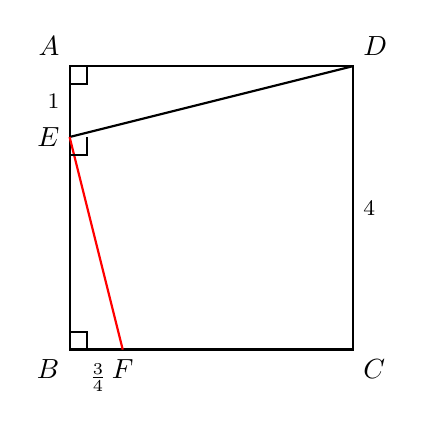
\begin{tikzpicture}[scale=0.9, thick]
  % 正方形：A 左上、B 左下、C 右下、D 右上？为了让 AB 是直线 l（含 E）
  % 题目：E∈AB, F∈BC. 把 AB 当作 l。让 A 上 B 下：A=(0,4), B=(0,0), C=(4,0), D=(4,4)
  \coordinate (A) at (0,4);
  \coordinate (B) at (0,0);
  \coordinate (C) at (4,0);
  \coordinate (D) at (4,4);
  \coordinate (E) at (0,3);  % AE=1
  \coordinate (F) at (0.75,0); % BF=3/4
  \draw (A)--(B)--(C)--(D)--cycle;
  \draw (D)--(E);
  \draw[red] (E)--(F);
  % 三直角
  \draw ($(A)+(0.25,0)$) -- ($(A)+(0.25,-0.25)$) -- ($(A)+(0,-0.25)$);
  \draw ($(B)+(0,0.25)$) -- ($(B)+(0.25,0.25)$) -- ($(B)+(0.25,0)$);
  % ∠DEF 直角
  \draw ($(E)+(0.25,0)$) -- ($(E)+(0.25,-0.25)$) -- ($(E)+(0,-0.25)$);
  \node[above left] at (A) {$A$};
  \node[below left] at (B) {$B$};
  \node[below right] at (C) {$C$};
  \node[above right] at (D) {$D$};
  \node[left] at (E) {$E$};
  \node[below] at (F) {$F$};
  \node[left] at ($(A)!0.5!(E)$) {\footnotesize $1$};
  \node[below] at (0.4,-0.05) {\footnotesize $\tfrac{3}{4}$};
  \node[right] at ($(C)!0.5!(D)$) {\footnotesize $4$};
\end{tikzpicture}
\end{document}
